\documentclass[11pt,addpoints,answers]{exam}
%\documentclass[11pt]{article}
\usepackage[margin=1in]{geometry}
\usepackage{amsmath, amsfonts}
\usepackage{enumerate}
\usepackage{graphicx}
\usepackage{titling}
\usepackage{url}
\usepackage{xfrac}
% \usepackage{fancyhdr} % CONFLICTS with the exam class
\usepackage{geometry}
\usepackage{graphicx}
\usepackage{natbib}
\usepackage{amsmath}
\usepackage{amssymb}
\usepackage{amsthm}
\usepackage{paralist}
\usepackage{epstopdf}
\usepackage{tabularx}
\usepackage{longtable}
\usepackage{multirow}
\usepackage{multicol}
\usepackage[colorlinks=true,urlcolor=blue]{hyperref}
\usepackage{fancyvrb}
\usepackage{algorithm}
\usepackage{algorithmic}
\usepackage{float}
\usepackage{paralist}
\usepackage[svgname]{xcolor}
\usepackage{enumerate}
\usepackage{array}
\usepackage{times}
\usepackage{url}
\usepackage{comment}
\usepackage{environ}
\usepackage{times}
\usepackage{textcomp}
\usepackage{caption}
\usepackage[colorlinks=true,urlcolor=blue]{hyperref}
\usepackage{listings}
\usepackage{parskip} % For NIPS style paragraphs.
\usepackage[compact]{titlesec} % Less whitespace around titles
\usepackage[inline]{enumitem} % For inline enumerate* and itemize*
\usepackage{datetime}
\usepackage{comment}
% \usepackage{minted}
\usepackage{lastpage}
\usepackage{color}
\usepackage{xcolor}
\usepackage{listings}
\usepackage{tikz}
\usetikzlibrary{shapes,decorations,bayesnet}
%\usepackage{framed}
\usepackage{booktabs}
\usepackage{cprotect}
\usepackage{xcolor}
\usepackage{verbatimbox}
\usepackage[many]{tcolorbox}
\usepackage{cancel}
\usepackage{wasysym}
\usepackage{mdframed}
\usepackage{subcaption}
\usetikzlibrary{shapes.geometric}
\usepackage[nomessages]{fp}

%%%%%%%%%%%%%%%%%%%%%%%%%%%%%%%%%%%%%%%%%%%
% Formatting for \CorrectChoice of "exam" %
%%%%%%%%%%%%%%%%%%%%%%%%%%%%%%%%%%%%%%%%%%%

\CorrectChoiceEmphasis{}
\checkedchar{\blackcircle}

%%%%%%%%%%%%%%%%%%%%%%%%%%%%%%%%%%%%%%%%%%%
% Better numbering                        %
%%%%%%%%%%%%%%%%%%%%%%%%%%%%%%%%%%%%%%%%%%%

\numberwithin{equation}{section} % Number equations within sections (i.e. 1.1, 1.2, 2.1, 2.2 instead of 1, 2, 3, 4)
\numberwithin{figure}{section} % Number figures within sections (i.e. 1.1, 1.2, 2.1, 2.2 instead of 1, 2, 3, 4)
\numberwithin{table}{section} % Number tables within sections (i.e. 1.1, 1.2, 2.1, 2.2 instead of 1, 2, 3, 4)


%%%%%%%%%%%%%%%%%%%%%%%%%%%%%%%%%%%%%%%%%%%
% Common Math Commands                    %
%%%%%%%%%%%%%%%%%%%%%%%%%%%%%%%%%%%%%%%%%%%

%%%%%%%%%%%%%%%%%%%%%%%%%%%%%%%%%%%%%%%%%%
% Custom commands                        %
%%%%%%%%%%%%%%%%%%%%%%%%%%%%%%%%%%%%%%%%%%

\newcommand{\vc}[1]{\boldsymbol{#1}}
\newcommand{\adj}[1]{\frac{d J}{d #1}}
\newcommand{\chain}[2]{\adj{#2} = \adj{#1}\frac{d #1}{d #2}}

% mathcal
\newcommand{\Ac}{\mathcal{A}}
\newcommand{\Bc}{\mathcal{B}}
\newcommand{\Cc}{\mathcal{C}}
\newcommand{\Dc}{\mathcal{D}}
\newcommand{\Ec}{\mathcal{E}}
\newcommand{\Fc}{\mathcal{F}}
\newcommand{\Gc}{\mathcal{G}}
\newcommand{\Hc}{\mathcal{H}}
\newcommand{\Ic}{\mathcal{I}}
\newcommand{\Jc}{\mathcal{J}}
\newcommand{\Kc}{\mathcal{K}}
\newcommand{\Lc}{\mathcal{L}}
\newcommand{\Mc}{\mathcal{M}}
\newcommand{\Nc}{\mathcal{N}}
\newcommand{\Oc}{\mathcal{O}}
\newcommand{\Pc}{\mathcal{P}}
\newcommand{\Qc}{\mathcal{Q}}
\newcommand{\Rc}{\mathcal{R}}
\newcommand{\Sc}{\mathcal{S}}
\newcommand{\Tc}{\mathcal{T}}
\newcommand{\Uc}{\mathcal{U}}
\newcommand{\Vc}{\mathcal{V}}
\newcommand{\Wc}{\mathcal{W}}
\newcommand{\Xc}{\mathcal{X}}
\newcommand{\Yc}{\mathcal{Y}}
\newcommand{\Zc}{\mathcal{Z}}

% mathbb
\newcommand{\Ab}{\mathbb{A}}
\newcommand{\Bb}{\mathbb{B}}
\newcommand{\Cb}{\mathbb{C}}
\newcommand{\Db}{\mathbb{D}}
\newcommand{\Eb}{\mathbb{E}}
\newcommand{\Fb}{\mathbb{F}}
\newcommand{\Gb}{\mathbb{G}}
\newcommand{\Hb}{\mathbb{H}}
\newcommand{\Ib}{\mathbb{I}}
\newcommand{\Jb}{\mathbb{J}}
\newcommand{\Kb}{\mathbb{K}}
\newcommand{\Lb}{\mathbb{L}}
\newcommand{\Mb}{\mathbb{M}}
\newcommand{\Nb}{\mathbb{N}}
\newcommand{\Ob}{\mathbb{O}}
\newcommand{\Pb}{\mathbb{P}}
\newcommand{\Qb}{\mathbb{Q}}
\newcommand{\Rb}{\mathbb{R}}
\newcommand{\Sb}{\mathbb{S}}
\newcommand{\Tb}{\mathbb{T}}
\newcommand{\Ub}{\mathbb{U}}
\newcommand{\Vb}{\mathbb{V}}
\newcommand{\Wb}{\mathbb{W}}
\newcommand{\Xb}{\mathbb{X}}
\newcommand{\Yb}{\mathbb{Y}}
\newcommand{\Zb}{\mathbb{Z}}

% mathbf lowercase
\newcommand{\av}{\mathbf{a}}
\newcommand{\bv}{\mathbf{b}}
\newcommand{\cv}{\mathbf{c}}
\newcommand{\dv}{\mathbf{d}}
\newcommand{\ev}{\mathbf{e}}
\newcommand{\fv}{\mathbf{f}}
\newcommand{\gv}{\mathbf{g}}
\newcommand{\hv}{\mathbf{h}}
\newcommand{\iv}{\mathbf{i}}
\newcommand{\jv}{\mathbf{j}}
\newcommand{\kv}{\mathbf{k}}
\newcommand{\lv}{\mathbf{l}}
\newcommand{\mv}{\mathbf{m}}
\newcommand{\nv}{\mathbf{n}}
\newcommand{\ov}{\mathbf{o}}
\newcommand{\pv}{\mathbf{p}}
\newcommand{\qv}{\mathbf{q}}
\newcommand{\rv}{\mathbf{r}}
\newcommand{\sv}{\mathbf{s}}
\newcommand{\tv}{\mathbf{t}}
\newcommand{\uv}{\mathbf{u}}
\newcommand{\vv}{\mathbf{v}}
\newcommand{\wv}{\mathbf{w}}
\newcommand{\xv}{\mathbf{x}}
\newcommand{\yv}{\mathbf{y}}
\newcommand{\zv}{\mathbf{z}}

% mathbf uppercase
\newcommand{\Av}{\mathbf{A}}
\newcommand{\Bv}{\mathbf{B}}
\newcommand{\Cv}{\mathbf{C}}
\newcommand{\Dv}{\mathbf{D}}
\newcommand{\Ev}{\mathbf{E}}
\newcommand{\Fv}{\mathbf{F}}
\newcommand{\Gv}{\mathbf{G}}
\newcommand{\Hv}{\mathbf{H}}
\newcommand{\Iv}{\mathbf{I}}
\newcommand{\Jv}{\mathbf{J}}
\newcommand{\Kv}{\mathbf{K}}
\newcommand{\Lv}{\mathbf{L}}
\newcommand{\Mv}{\mathbf{M}}
\newcommand{\Nv}{\mathbf{N}}
\newcommand{\Ov}{\mathbf{O}}
\newcommand{\Pv}{\mathbf{P}}
\newcommand{\Qv}{\mathbf{Q}}
\newcommand{\Rv}{\mathbf{R}}
\newcommand{\Sv}{\mathbf{S}}
\newcommand{\Tv}{\mathbf{T}}
\newcommand{\Uv}{\mathbf{U}}
\newcommand{\Vv}{\mathbf{V}}
\newcommand{\Wv}{\mathbf{W}}
\newcommand{\Xv}{\mathbf{X}}
\newcommand{\Yv}{\mathbf{Y}}
\newcommand{\Zv}{\mathbf{Z}}

% bold greek lowercase
\newcommand{\alphav     }{\boldsymbol \alpha     }
\newcommand{\betav      }{\boldsymbol \beta      }
\newcommand{\gammav     }{\boldsymbol \gamma     }
\newcommand{\deltav     }{\boldsymbol \delta     }
\newcommand{\epsilonv   }{\boldsymbol \epsilon   }
\newcommand{\varepsilonv}{\boldsymbol \varepsilon}
\newcommand{\zetav      }{\boldsymbol \zeta      }
\newcommand{\etav       }{\boldsymbol \eta       }
\newcommand{\thetav     }{\boldsymbol \theta     }
\newcommand{\varthetav  }{\boldsymbol \vartheta  }
\newcommand{\iotav      }{\boldsymbol \iota      }
\newcommand{\kappav     }{\boldsymbol \kappa     }
\newcommand{\varkappav  }{\boldsymbol \varkappa  }
\newcommand{\lambdav    }{\boldsymbol \lambda    }
\newcommand{\muv        }{\boldsymbol \mu        }
\newcommand{\nuv        }{\boldsymbol \nu        }
\newcommand{\xiv        }{\boldsymbol \xi        }
\newcommand{\omicronv   }{\boldsymbol \omicron   }
\newcommand{\piv        }{\boldsymbol \pi        }
\newcommand{\varpiv     }{\boldsymbol \varpi     }
\newcommand{\rhov       }{\boldsymbol \rho       }
\newcommand{\varrhov    }{\boldsymbol \varrho    }
\newcommand{\sigmav     }{\boldsymbol \sigma     }
\newcommand{\varsigmav  }{\boldsymbol \varsigma  }
\newcommand{\tauv       }{\boldsymbol \tau       }
\newcommand{\upsilonv   }{\boldsymbol \upsilon   }
\newcommand{\phiv       }{\boldsymbol \phi       }
\newcommand{\varphiv    }{\boldsymbol \varphi    }
\newcommand{\chiv       }{\boldsymbol \chi       }
\newcommand{\psiv       }{\boldsymbol \psi       }
\newcommand{\omegav     }{\boldsymbol \omega     }

% bold greek uppercase
\newcommand{\Gammav     }{\boldsymbol \Gamma     }
\newcommand{\Deltav     }{\boldsymbol \Delta     }
\newcommand{\Thetav     }{\boldsymbol \Theta     }
\newcommand{\Lambdav    }{\boldsymbol \Lambda    }
\newcommand{\Xiv        }{\boldsymbol \Xi        }
\newcommand{\Piv        }{\boldsymbol \Pi        }
\newcommand{\Sigmav     }{\boldsymbol \Sigma     }
\newcommand{\Upsilonv   }{\boldsymbol \Upsilon   }
\newcommand{\Phiv       }{\boldsymbol \Phi       }
\newcommand{\Psiv       }{\boldsymbol \Psi       }
\newcommand{\Omegav     }{\boldsymbol \Omega     }


%%%%%%%%%%%%%%%%%%%%%%%%%%%%%%%%%%%%%%%%%%%
% Code highlighting with listings         %
%%%%%%%%%%%%%%%%%%%%%%%%%%%%%%%%%%%%%%%%%%%

\definecolor{bluekeywords}{rgb}{0.13,0.13,1}
\definecolor{greencomments}{rgb}{0,0.5,0}
\definecolor{redstrings}{rgb}{0.9,0,0}
\definecolor{light-gray}{gray}{0.95}

\newcommand{\MYhref}[3][blue]{\href{#2}{\color{#1}{#3}}}%

\definecolor{dkgreen}{rgb}{0,0.6,0}
\definecolor{gray}{rgb}{0.5,0.5,0.5}
\definecolor{mauve}{rgb}{0.58,0,0.82}

\lstdefinelanguage{Shell}{
  keywords={tar, cd, make},
  %keywordstyle=\color{bluekeywords}\bfseries,
  alsoletter={+},
  ndkeywords={python, py, javac, java, gcc, c, g++, cpp, .txt, octave, m, .tar},
  %ndkeywordstyle=\color{bluekeywords}\bfseries,
  identifierstyle=\color{black},
  sensitive=false,
  comment=[l]{//},
  morecomment=[s]{/*}{*/},
  commentstyle=\color{purple}\ttfamily,
  stringstyle=\color{red}\ttfamily,
  morestring=[b]',
  morestring=[b]",
  backgroundcolor = \color{light-gray}
}

\lstset{columns=fixed, basicstyle=\ttfamily,
    backgroundcolor=\color{light-gray},xleftmargin=0.5cm,frame=tlbr,framesep=4pt,framerule=0pt}


%%%%%%%%%%%%%%%%%%%%%%%%%%%%%%%%%%%%%%%%%%%
% Custom box for highlights               %
%%%%%%%%%%%%%%%%%%%%%%%%%%%%%%%%%%%%%%%%%%%

% Define box and box title style
\tikzstyle{mybox} = [fill=blue!10, very thick,
    rectangle, rounded corners, inner sep=1em, inner ysep=1em]

% \newcommand{\notebox}[1]{
% \begin{tikzpicture}
% \node [mybox] (box){%
%     \begin{minipage}{\textwidth}
%     #1
%     \end{minipage}
% };
% \end{tikzpicture}%
% }

\NewEnviron{notebox}{
\begin{tikzpicture}
\node [mybox] (box){
    \begin{minipage}{\textwidth}
        \BODY
    \end{minipage}
};
\end{tikzpicture}
}

%%%%%%%%%%%%%%%%%%%%%%%%%%%%%%%%%%%%%%%%%%%
% Commands showing / hiding solutions     %
%%%%%%%%%%%%%%%%%%%%%%%%%%%%%%%%%%%%%%%%%%%

%% To HIDE SOLUTIONS (to post at the website for students), set this value to 0: \def\issoln{0}
\def\issoln{0}
% Some commands to allow solutions to be embedded in the assignment file.
\ifcsname issoln\endcsname \else \def\issoln{0} \fi
% Default to an empty solutions environ.
\NewEnviron{soln}{}{}
% Default to an empty qauthor environ.
\NewEnviron{qauthor}{}{}
% Default to visible (but empty) solution box.
\newtcolorbox[]{studentsolution}[1][]{%
    breakable,
    enhanced,
    colback=white,
    title=Solution,
    #1
}

\if\issoln 1
% Otherwise, include solutions as below.
\RenewEnviron{soln}{
    \leavevmode\color{red}\ignorespaces
    \textbf{Solution} \BODY
}{}
\fi

\if\issoln 1
% Otherwise, include solutions as below.
\RenewEnviron{solution}{}
\fi

%%%%%%%%%%%%%%%%%%%%%%%%%%%%%%%%%%%%%%%%%%%
% Commands for customizing the assignment %
%%%%%%%%%%%%%%%%%%%%%%%%%%%%%%%%%%%%%%%%%%%

\newcommand{\courseNum}{10-418 / 10-618}
\newcommand{\courseName}{Machine Learning for Structured Data}
\newcommand{\courseSem}{Fall 2019}
\newcommand{\piazzaUrl}{\url{https://piazza.com/cmu/fall2019/1041810618}}
\newcommand{\hwNum}{Homework 5}
\newcommand{\hwTopic}{Variational Inference}
\newcommand{\hwName}{\hwNum: \hwTopic}
\newcommand{\outDate}{Nov. 20, 2019}
\newcommand{\dueDate}{Dec 02, 2019 11:59 PM}
\newcommand{\taNames}{Aakanksha, Austin, Karthika}

\newcommand{\recentChange}[1]{{\color{red}#1}}

%\pagestyle{fancyplain}
\lhead{\hwName}
\rhead{\courseNum}
\cfoot{\thepage{} of \numpages{}}

\title{\textsc{\hwName}} % Title


\author{\courseName\\
  Carnegie Mellon University \\
\url{piazza.com/cmu/fall2018/10606607} \\
OUT: \outDate{}\thanks{Compiled on \today{} at \currenttime{}} \\
DUE: \dueDate{} \\ 
TAs: Aakanksha, Edgar, Sida, Varsha}

\date{}

%%%%%%%%%%%%%%%%%%%%%%%%%%%%%%%%%%%%%%%%%%%%%%%%%
% Useful commands for typesetting the questions %
%%%%%%%%%%%%%%%%%%%%%%%%%%%%%%%%%%%%%%%%%%%%%%%%%

\newcommand \expect {\mathbb{E}}
\newcommand \mle [1]{{\hat #1}^{\rm MLE}}
\newcommand \map [1]{{\hat #1}^{\rm MAP}}
\newcommand \argmax {\operatorname*{argmax}}
\newcommand \argmin {\operatorname*{argmin}}
\newcommand \code [1]{{\tt #1}}
\newcommand \datacount [1]{\#\{#1\}}
\newcommand \ind [1]{\mathbb{I}\{#1\}}

\newcommand{\blackcircle}{\tikz\draw[black,fill=black] (0,0) circle (1ex);}
\renewcommand{\circle}{\tikz\draw[black] (0,0) circle (1ex);}

\newcommand{\pts}[1]{\textbf{[#1 pts]}}

%%%%%%%%%%%%%%%%%%%%%%%%%%
% Document configuration %
%%%%%%%%%%%%%%%%%%%%%%%%%%

% Don't display a date in the title and remove the white space
\predate{}
\postdate{}
\date{}

% Don't display an author and remove the white space
%\preauthor{}
%\postauthor{}

%%%%%%%%%%%%%%%%%%
% Begin Document %
%%%%%%%%%%%%%%%%%% 


\begin{document}

\section*{}
\begin{center}
  \textsc{\LARGE \hwNum} \\
  \textsc{\LARGE \hwTopic\footnote{Compiled on \today{} at \currenttime{}}} \\
  \vspace{1em}
  \textsc{\large \courseNum{} \courseName{} (\courseSem)} \\
  %\vspace{0.25em}
  \piazzaUrl\\
  \vspace{1em}
  OUT: \outDate \\
  %\vspace{0.5em}
  DUE: \dueDate \\
  TAs: \taNames
\end{center}


\section*{START HERE: Instructions}

%\vspace{-1em}
\begin{notebox}
\paragraph{Summary} In this assignment, we will walk through the basics of Variational Inference, Mean-Field Approximation and the Coordinate Ascent Variational Inference (CAVI) algorithm for simple distributions such as multivariate Gaussians and Gaussian Mixture Models. Finally, we will wrap up with a brief comparison between variational methods and sampling-based methods such as MCMC.
\end{notebox}

\begin{itemize}
\item \textbf{Collaboration policy:} Collaboration on solving the homework is allowed, after you have thought about the problems on your own. It is also OK to get clarification (but not solutions) from books or online resources, again after you have thought about the problems on your own. There are two requirements: first, cite your collaborators fully and completely (e.g., ``Jane explained to me what is asked in Question 2.1''). Second, write your solution {\em independently}: close the book and all of your notes, and send collaborators out of the room, so that the solution comes from you only.  See the Academic Integrity Section on the course site for more information: \url{http://www.cs.cmu.edu/~mgormley/courses/10418/about.html#7-academic-integrity-policies}

\item\textbf{Late Submission Policy:} See the late submission policy here: \url{http://www.cs.cmu.edu/~mgormley/courses/10418/about.html#6-general-policies}


\item \textbf{Autolab:} You will submit your code for programming questions on the homework to Autolab (\url{https://autolab.andrew.cmu.edu/}). After uploading your code,
we will manually grade your code by hand. We will not use Autolab to autograde your code.

\item \textbf{Submitting your work to Gradescope:} For written problems such as short answer, multiple choice, derivations, proofs, or plots, we will be using Gradescope (\url{https://gradescope.com/}). Please use the provided template. Submissions can be handwritten, but should be labeled and clearly legible. If your writing is not legible, you will not be awarded marks. Alternatively, submissions can be written in LaTeX. Regrade requests can be made, however this gives the TA the opportunity to regrade your entire paper, meaning if additional mistakes are found then points will be deducted. For short answer questions you \textbf{should not} include your work in your solution.  If you include your work in your solutions, your assignment may not be graded correctly by our AI assisted grader. 

\end{itemize}

For multiple choice or select all that apply questions, shade in the box or circle in the template document corresponding to the correct answer(s) for each of the questions. For \LaTeX{} users, replace \lstinline{\choice} with \lstinline{\CorrectChoice} to obtain a shaded box/circle, and don't change anything else.


\clearpage

\section{Written Questions \pts{\numpoints{}}}
\label{sec:warmup}
Answer the following questions in the template provided.  Then upload your solutions to Gradescope. You may use \LaTeX\ or print the template and hand-write your answers then scan it in. Failure to use the template may result in a penalty. There are \numpoints{} points and \numquestions{} questions.

\subsection{Mean-Field Approximation for Multivariate Gaussians}

In this question, we'll explore how accurate a Mean-Field approximation can be for an underlying multivariate Gaussian distribution. 

Assume we have observed data $\Xv = \{\xv^{(i)}\}_{i=1}^n$ that was drawn from a 2-dimensional Gaussian distribution $p(\xv; \muv, \ \Lambdav^{-1})$. 

\begin{equation}
    p(\xv; \muv, \ \Lambdav) = \mathcal{N}\bigg ( 
    \begin{pmatrix}
    x_1 \\
    x_2 \\
    \end{pmatrix} ;
    \begin{pmatrix}
    \mu_1 \\
    \mu_2
    \end{pmatrix}, 
    \begin{pmatrix}
    \Lambda_{11} & \Lambda_{12} \\
    \Lambda_{21} & \Lambda_{22} \\
    \end{pmatrix}^{-1}
    \bigg )
\end{equation}

Note here that we're using the \textit{precision} matrix $\Lambdav = \Sigmav^{-1}$. An additional property of the precision matrix is that it is symmetric, so $\Lambda_{12} = \Lambda_{21}$. This will make your lives easier for the math to come. 

We will approximate this 2-dimensional Gaussian with a mean field approximation, $q(\xv) = q(\xv_1)q(\xv_2)$, the product of two 1-dimensional distributions $q(\xv_1)$ and $q(\xv_2)$. For now, we won't assume any form for this distributions. 

\begin{questions}
\question[1] \textbf{Short Answer:} Write down the equation for $\log p(\Xv)$. For now, you can leave all of the parameters in terms of vectors and matrices, not their subcomponents. 

\begin{tcolorbox}[fit,height=2cm, width=15cm, blank, borderline={1pt}{-2pt}]
% STUDENT SOLUTION HERE
\end{tcolorbox}

\question[2] \textbf{Short Answer:} Group together everything that involves $\Xv_1$ and remove anything involving $\Xv_2$. We claim that there exists some distribution $q^*(\Xv) = q^*(\Xv_1)q^*(\Xv_2)$ that minimizes the KL divergence  $q^* = \argmin_{q} \text{KL}(q || p)$. And further, said distribution will have a component $q^\star(\Xv_1)$ will be proportional to the quantity you find below.  

\begin{tcolorbox}[fit,height=2cm, width=15cm, blank, borderline={1pt}{-2pt}]
% STUDENT SOLUTION HERE
\end{tcolorbox}

It can be shown that this implies that $q(\Xv_1)$ (and therefore $q(\Xv_2)$) is a Gaussian distribution. 

\begin{equation*}
    q(\xv_1) = \mathcal{N}(\xv_1; m_1, \Lambda_{11}^{-1})
\end{equation*}

Where $m_1 = \mu_1 - \Lambda_{11}^{-1}\Lambda_{12}(\mathbb{E}[x_2]-\mu_2)$

Using these facts, we'd like to explore how well our approximation can model the underlying distribution. 

\question Suppose the parameters of the true distribution are $\muv = \begin{pmatrix} 0 \\ 0 \end{pmatrix}$ and $\Lambdav = \begin{pmatrix} 1 & 0 \\ 0 & 1/4 \end{pmatrix}$. 

\begin{parts}

\part[1] \textbf{Numerical Answer:} What is the value of the mean of the Gaussian for $q^*(\Xv_1)$?
    \begin{tcolorbox}[fit,height=1cm, width=2cm, blank, borderline={1pt}{-2pt}]
    \end{tcolorbox}
    
\part[1] \textbf{Numerical Answer:} What is the value of the variance of the Gaussian for $q^*(\Xv_1)$?
    \begin{tcolorbox}[fit,height=1cm, width=2cm, blank, borderline={1pt}{-2pt}]
    \end{tcolorbox}
    
\part[1] \textbf{Numerical Answer:} What is the value of the mean of the Gaussian for $q^*(\Xv_2)$?
    \begin{tcolorbox}[fit,height=1cm, width=2cm, blank, borderline={1pt}{-2pt}]
    \end{tcolorbox}
    
\part[1] \textbf{Numerical Answer:} What is the value of the variance of the Gaussian for $q^*(\Xv_2)$?
    \begin{tcolorbox}[fit,height=1cm, width=2cm, blank, borderline={1pt}{-2pt}]
    \end{tcolorbox}

\part[2] \textbf{Plot:} Provide a \emph{computer-generated} contour plot to show the result of our approximation $q^*(\Xv)$ and the true underlying Gaussian $p(\Xv; \muv, \Lambdav)$ for the parameters given above.
    \begin{tcolorbox}[fit,height=8cm, width=15cm, blank, borderline={1pt}{-2pt}]
    \end{tcolorbox}

\end{parts}

\question Suppose the parameters of the true distribution are $\muv = \begin{pmatrix} 1 \\ 2 \end{pmatrix}$ and $\Lambdav = \begin{pmatrix} 1 & -3 \\ 0 & 1 \end{pmatrix}$. 

\begin{parts}

\part[1] \textbf{Numerical Answer:} What is the value of the mean of the Gaussian for $q^*(\Xv_1)$?
    \begin{tcolorbox}[fit,height=1cm, width=2cm, blank, borderline={1pt}{-2pt}]
    \end{tcolorbox}
    
\part[1] \textbf{Numerical Answer:} What is the value of the variance of the Gaussian for $q^*(\Xv_1)$?
    \begin{tcolorbox}[fit,height=1cm, width=2cm, blank, borderline={1pt}{-2pt}]
    \end{tcolorbox}
    
\part[1] \textbf{Numerical Answer:} What is the value of the mean of the Gaussian for $q^*(\Xv_2)$?
    \begin{tcolorbox}[fit,height=1cm, width=2cm, blank, borderline={1pt}{-2pt}]
    \end{tcolorbox}
    
\part[1] \textbf{Numerical Answer:} What is the value of the variance of the Gaussian for $q^*(\Xv_2)$?
    \begin{tcolorbox}[fit,height=1cm, width=2cm, blank, borderline={1pt}{-2pt}]
    \end{tcolorbox}

\part[2] \textbf{Plot:} Provide a \emph{computer-generated} contour plot to show the result of our approximation $q^*(\Xv)$ and the true underlying Gaussian $p(\Xv; \muv, \Lambdav)$ for the parameters given above.
    \begin{tcolorbox}[fit,height=8cm, width=15cm, blank, borderline={1pt}{-2pt}]
    \end{tcolorbox}

\end{parts}

\question[1] Describe in words how the plots you generated provide insight into the behavior of minimization of $KL(q||p)$ with regards to the low probability and high probability regions of the the true vs. approximate distributions.

\begin{tcolorbox}[fit,height=4cm, width=15cm, blank, borderline={1pt}{-2pt}]
\end{tcolorbox}

\end{questions}{}

\subsection{Variational Inference for Gaussian Mixture Models}
Now that we have seen how the mean-field approximation works for a multivariate Gaussian, let's look at the case of Gaussian Mixture Models. Suppose we have a Bayesian mixture of unit-variance univariate Gaussian distributions. This mixture consists of 2 components each corresponding to a Gaussian distribution, with means $\muv = \{\mu_1,\mu_2\}$. The mean parameters are drawn independently from a Gaussian prior distribution $\mathcal{N}(0, \sigma^2)$. The prior variance $\sigma^2$ is a hyperparameter. Generating an observation $x_i$ from this model is done according to the following generative story:
\begin{enumerate}
    \item Choose a cluster assignment $c_i$ for the observation. The cluster assignment is chosen from the distribution Categorical$(\frac{1}{2}, \frac{1}{2})$ and indicates which latent cluster $x_i$ comes from. Encode $c_i$ as a one-hot vector where $[1,0]$ indicates that $x_i$ is assigned to cluster 0 and vice versa.
    \item Generate $x_i$ from the corresponding Gaussian distribution $\mathcal{N}(c_i^T\muv, 1)$
\end{enumerate}
The complete hierarchical model is as follows:
\begin{align*}
    \mu_k &\sim \mathcal{N}(0, \sigma^2), k \in \{1,2\}\\
    c_i &\sim \text{Categorical}(\frac{1}{2}, \frac{1}{2}), i \in [1,n]\\
    x_i | c_i, \muv &\sim \mathcal{N}(c_i^T\muv, 1), i \in [1,n] 
\end{align*}
where n is the number of observations generated from the model.

\begin{questions}
\question[1] What are the observed and latent variables for this model?
\begin{tcolorbox}[fit,height=2cm, width=15cm, blank, borderline={1pt}{-2pt}]
% STUDENT SOLUTION HERE
\end{tcolorbox}

\question[1] Write down the joint probability of observed and latent variables under this model
\begin{tcolorbox}[fit,height=2cm, width=15cm, blank, borderline={1pt}{-2pt}]
% STUDENT SOLUTION HERE
\end{tcolorbox}

\question[3] Let's calculate the ELBO (evidence lower-bound) for this model. Recall that the ELBO is given by the following equation:
\begin{align*}
    \text{ELBO}(q) = \mathbb{E}_q[\log p(\xv, \zv)] - \mathbb{E}_q[\log q(\zv)]
\end{align*}
To calculate $q(\zv)$, we will now use the mean-field assumption. Under this assumption, each latent variable is governed by its own latent factor, resulting in the following probability distribution:
\begin{align*}
    q(\muv, \cv) &= \left( \prod_{k=1}^2 q(\mu_k; m_k, v_k^2) \right) \left( \prod_{i=1}^n q(c_i; a_i) \right)
\end{align*}
Here $q(\mu_k; m_k, v_k^2)$ is the Gaussian distribution for the $k$-th mixture component with mean and variance $m_k$ and $v_k^2$. $q(c_i; a_i)$ is the categorical distribution for the $i$-th observation with assignment probabilities $a_i$ ($a_i$ is a 2-dimensional vector). Given this assumption, write down the ELBO as a function of the variational parameters $\mv, \vv^2, \av$.

\begin{tcolorbox}[fit,height=4cm, width=15cm, blank, borderline={1pt}{-2pt}]
% STUDENT SOLUTION HERE
\end{tcolorbox}

\question Now that we have the ELBO formulation, let's try to compute coordinate updates for our latent variables. Remember that the optimal variational density of a latent variable $z_i$ is proportional to the exponentiated expected log of the complete conditional given all other latent variables in the model and the observed data. In other words:
\begin{align*}
    q_i(z_i) &\propto \exp{\Bigg(\mathbb{E}_{-j}[\log p(z_j | \zv_{-j}, \xv)]\Bigg)}
\end{align*}
Equivalently, you can also say that the variational density is proportional to the exponentiated expected log of the joint $\mathbb{E}_{-j}[\log p(z_j, \zv_{-j}, \xv)]$. This is a valid coordinate update since the expectations on the right side of the equation do not involve $z_j$ due to the mean-field assumption. 
\begin{parts}
\part[4] Show that the variational update for $a_{i1} \propto exp\Bigg(\mathbb{E}[\mu_1; m_1, s_1^2]x_i - \frac{\mathbb{E}[\mu_1; m_1, s_1^2]}{2} \Bigg)$. \\ (\textbf{Hint:} We can write the optimal variational density for cluster assignment variables as \\
$q(c_i;a_{i1}) \propto \exp{\Bigg( \log p(c_i) + \mathbb{E}_{\muv}[\log p(x_i | c_i, \muv); \mv, \vv^2] \Bigg)}$. Feel free to drop added constants along the way.)

\begin{tcolorbox}[fit,height=10cm, width=15cm, blank, borderline={1pt}{-2pt}]
% STUDENT SOLUTION HERE
\end{tcolorbox}

\part[6] Show that the variational updates for the $k$-th mixture component are $m_k = \frac{\sum_i a_{ik} x_i}{1/\sigma^2 + \sum_i a_{ik}}$ and $v_k = \frac{1}{1/\sigma^2 + \sum_i a_{ik}}$.\\ (\textbf{Hint:} We can write the optimal variational density for the $k$-th mixture component as\\ $q(\mu_k) \propto \exp{\Bigg( \log p(\mu_k) + \mathbb{E}_{c_i}[\log p(x_i | c_i, \muv); a_i, \mv_{-k}, \vv_{-k}^2] \Bigg)}$. Feel free to drop added constants along the way.)

\begin{tcolorbox}[fit,height=10cm, width=15cm, blank, borderline={1pt}{-2pt}]
% STUDENT SOLUTION HERE
\end{tcolorbox}

\end{parts}

\end{questions}

\subsection{Running CAVI: Toy Example}
Let's now see this in action!

Recall that the CAVI update algorithm for a Gaussian Mixture Model is as follows:
\begin{center}
    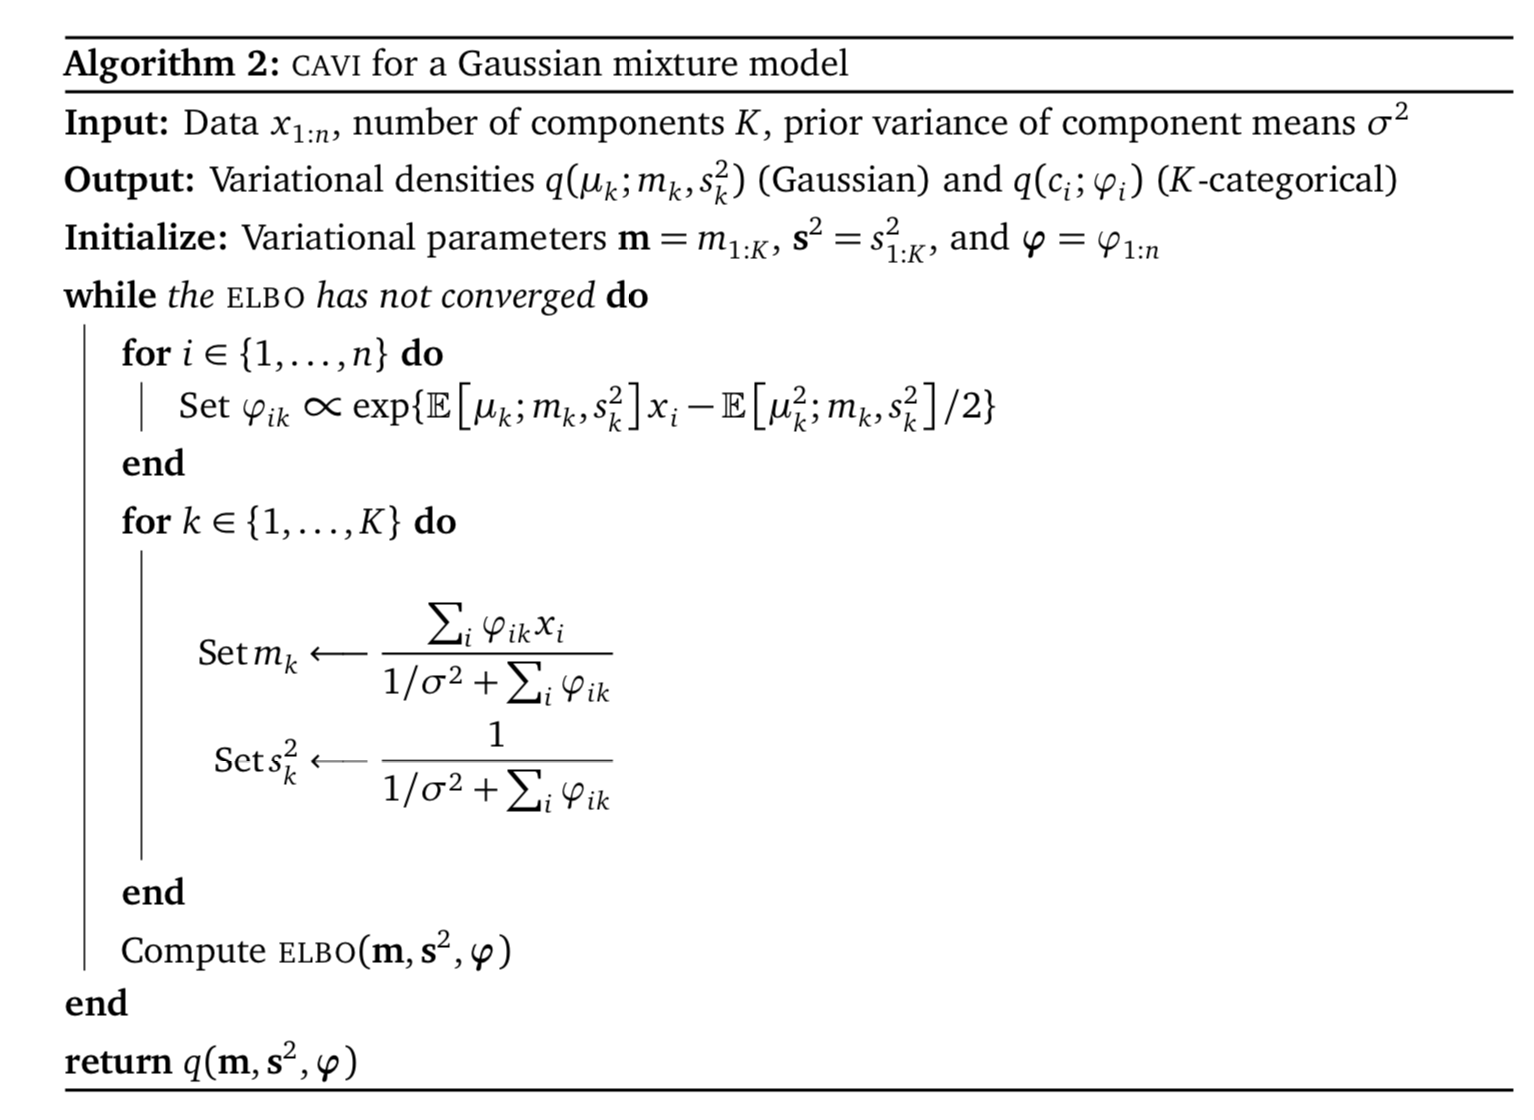
\includegraphics[width=0.70\columnwidth]{figures/cavi.png}

\end{center}
Note that our notation differs slightly, with $\varphi$ corresponding to $a$ and $s^2$ corresponding to $v^2$. We also have $K=2$.
Assume initial parameters, 
$\mv = [0.5,0.5]$, $
\vv^2 = [1,1]$ and $a_i= [0.3,0.7]$ for all $i \in n$ and a sample $x = [0.1,-0.3,1.2,0.8,-0.5]$. Also assume prior variance $\sigma^2 = 0.01$

Write a python script implementing the above procedure and run it for 5 epochs. You should submit your code to autolab as a .tar file named cavi.tar containing a single file cavi.py.
You can create that file by running:
\begin{lstlisting}
tar -cvf cavi.tar cavi.py
\end{lstlisting}
from the directory containing your code.

After the fifth epoch, report
\begin{questions}
\question[2] The variational parameters $\mv$.
\begin{center}
 \begin{tabular}{ |c|p{2cm}|p{2cm}|} 
 \hline
 \textbf{$\mv$} & & \\
 \hline
 
\end{tabular}
\end{center}


\question[2] The variational parameters $\vv^2$.
\begin{center}
 \begin{tabular}{ |c|p{2cm}|p{2cm}|} 
 \hline
 \textbf{$\vv^2$} & & \\
 \hline
 
\end{tabular}
\end{center}
\question[2] The variational parameters $\av$.
\begin{center}
 \begin{tabular}{ |c|p{2cm}|p{2cm}|} 
 \hline
 \textbf{$a_1$} & & \\
 \hline
 \textbf{$a_2$} & & \\
 \hline
 \textbf{$a_3$} & & \\
 \hline
 \textbf{$a_4$} & & \\
 \hline
 \textbf{$a_5$} & & \\
 \hline
 
\end{tabular}
\end{center}

\textbf{Hint:} 
\begin{enumerate}
    \item Note that the expectation update for $\av$ does not depend on $\mu$. (Why?)
    \item The expectation of the square of a Gaussian random variable is $\mathbb{E}[X^2] = Var[X] + \mathbb{E}([X])^2$.
\end{enumerate}
\end{questions}{}

\subsection{Variational Inference vs. Monte Carlo Methods}
Let's end with a brief comparison between variational methods and MCMC methods. We have seen that both classes of methods can be used for learning in scenarios involving latent variables, but both have their own sets of advantages and disadvantages. For each of the following statements, specify whether they apply more suitably to VI or MCMC methods:

\begin{questions}
\question[1]  Transforms inference into optimization problems.

\begin{checkboxes}
     \choice Variational Inference
     \choice MCMC
\end{checkboxes}

\question[1] Is easier to integrate with back-propagation.

\begin{checkboxes}
     \choice Variational Inference
     \choice MCMC
\end{checkboxes}

\question[1] Involves more stochasticity.

\begin{checkboxes}
     \choice Variational Inference
     \choice MCMC
\end{checkboxes}
 
  
\question[1] Non-parametric.  

\begin{checkboxes}
     \choice Variational Inference
     \choice MCMC
\end{checkboxes}


      
\question[1] Is higher variance under limited computational resources.

\begin{checkboxes}
     \choice Variational Inference
     \choice MCMC
\end{checkboxes}
       
     
% --
\end{questions}
\subsection{Wrap-up Questions}

\begin{questions}

\question[1] \textbf{Multiple Choice:} Did you correctly submit your code to Autolab? 
    \begin{checkboxes}
     \choice Yes 
     \choice No
    \end{checkboxes}

\question[1] \textbf{Numerical answer:} How many hours did you spend on this assignment?.
    \begin{tcolorbox}[fit,height=1cm, width=2cm, blank, borderline={1pt}{-2pt}]
    % STUDENT SOLUTION HERE
    \end{tcolorbox}

\end{questions}

\clearpage
\subsection{Collaboration Policy}

    After you have completed all other components of this assignment, report your answers to the collaboration policy questions detailed in the Academic Integrity Policies for this course.
    \begin{enumerate}
        \item Did you receive any help whatsoever from anyone in solving this assignment? If so, include full details including names of people who helped you and the exact nature of help you received.
        
        \begin{tcolorbox}[fit,height=4cm, width=15cm, blank, borderline={1pt}{-2pt},nobeforeafter]
        % Place your solution between the comment lines below.
        % Do not modify the tcolorbox.
        % ----------------------------------------------------
        % STUDENT SOLUTION HERE
        % ----------------------------------------------------
       \end{tcolorbox}
        \item Did you give any help whatsoever to anyone in solving this assignment? If so, include full details including names of people you helped and the exact nature of help you offered.
        
        \begin{tcolorbox}[fit,height=4cm, width=15cm, blank, borderline={1pt}{-2pt},nobeforeafter]
        % Place your solution between the comment lines below.
        % Do not modify the tcolorbox.
        % ----------------------------------------------------
        % STUDENT SOLUTION HERE
        % ----------------------------------------------------
       \end{tcolorbox}
        \item Did you find or come across code that implements any part of this assignment? If so, include full details including the source of the code and how you used it in the assignment.
        
        \begin{tcolorbox}[fit,height=4cm, width=15cm, blank, borderline={1pt}{-2pt},nobeforeafter]
        % Place your solution between the comment lines below.
        % Do not modify the tcolorbox.
        % ----------------------------------------------------
        % STUDENT SOLUTION HERE
        % ----------------------------------------------------
       \end{tcolorbox}
    \end{enumerate}

\end{document}